\documentclass{standalone}
\usepackage{helvet}
\renewcommand{\familydefault}{\sfdefault}
\usepackage{graphicx}
\graphicspath{
  {/home/sshin/git/shin-faculty-applications/},
  {/home/sshin/git/shin-faculty-applications/fig/},
  {/home/sshin/git/shin-faculty-applications/fig/old/},
  {/home/sshin/git/shin-faculty-applications/fig/nw-people/}
}
\usepackage{tikz}
\begin{document}
\begin{tikzpicture}[align=center,font=\footnotesize]
  \node at (0,1) {
    Energy Infrastructures\\[.5em]
    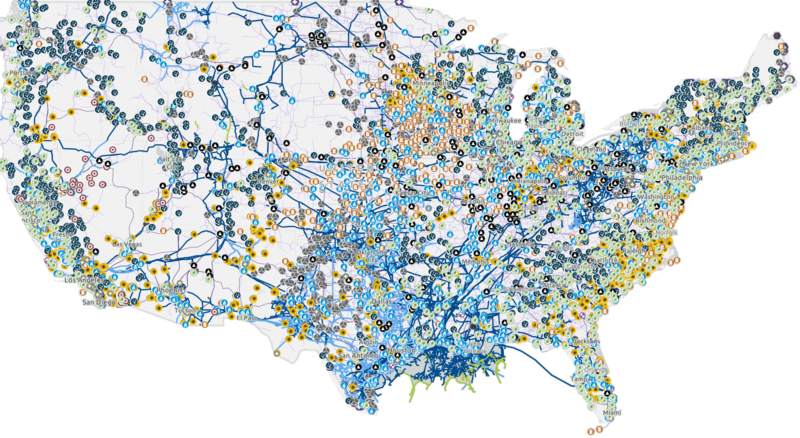
\includegraphics[width=200pt]{map-old.png}
  };
  \node at (0,-1.5) {
    Emerging Technologies
  };
  \node at (-2.7,-2.7) {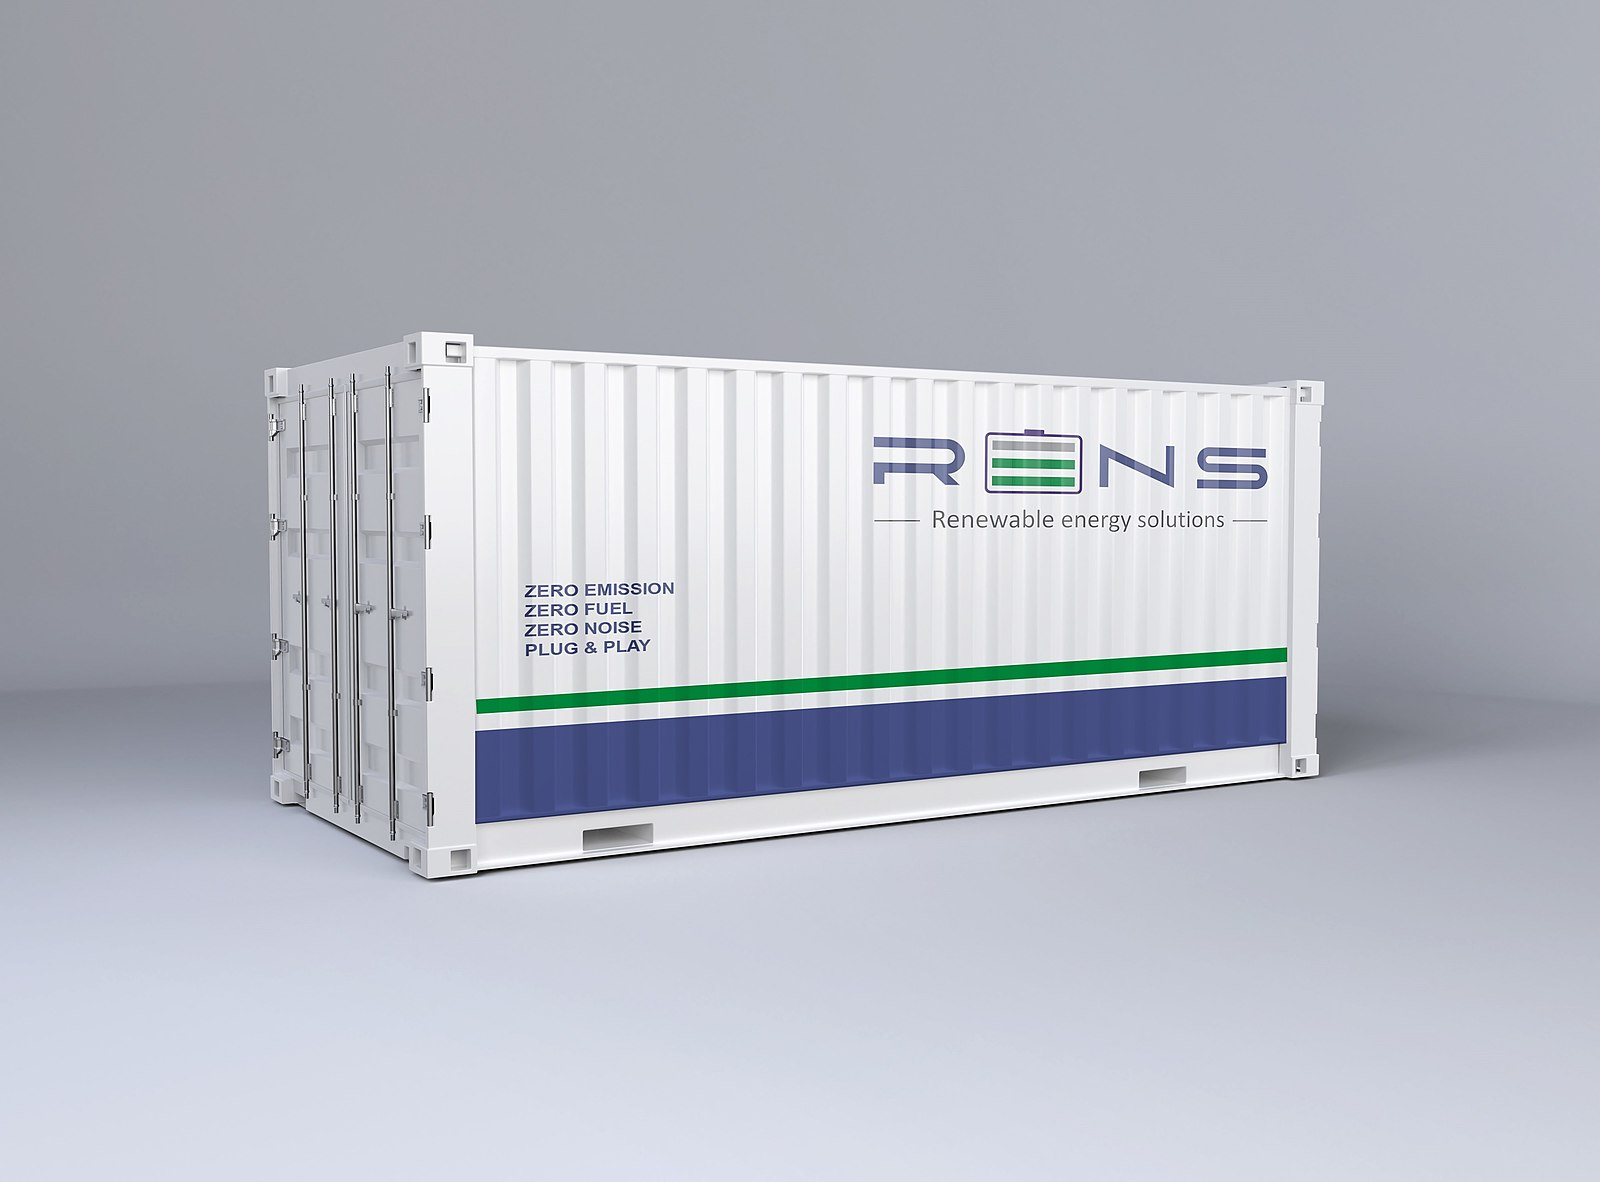
\includegraphics[width=76pt,height=46pt]{battery.jpg}};
  \node at (0,-2.7) {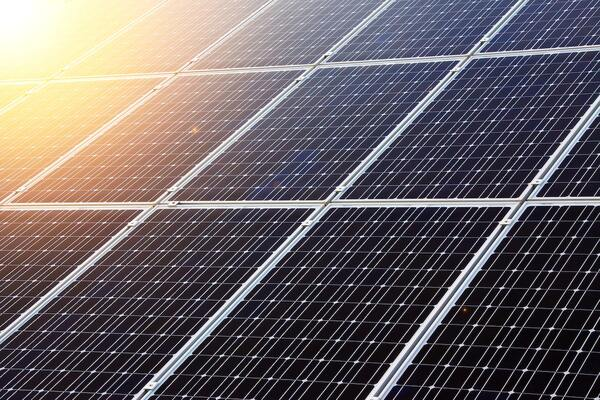
\includegraphics[width=76pt,height=46pt]{solar.jpg}};
  \node at (2.7,-2.7) {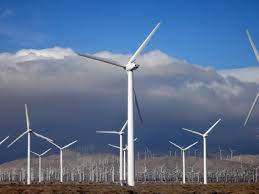
\includegraphics[width=76pt,height=46pt]{wind.jpg}};
  \node at (-2.7,-4.35) {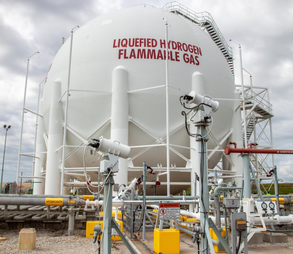
\includegraphics[width=76pt,height=46pt]{hydrogen.png}};
  \node at (0,-4.35) {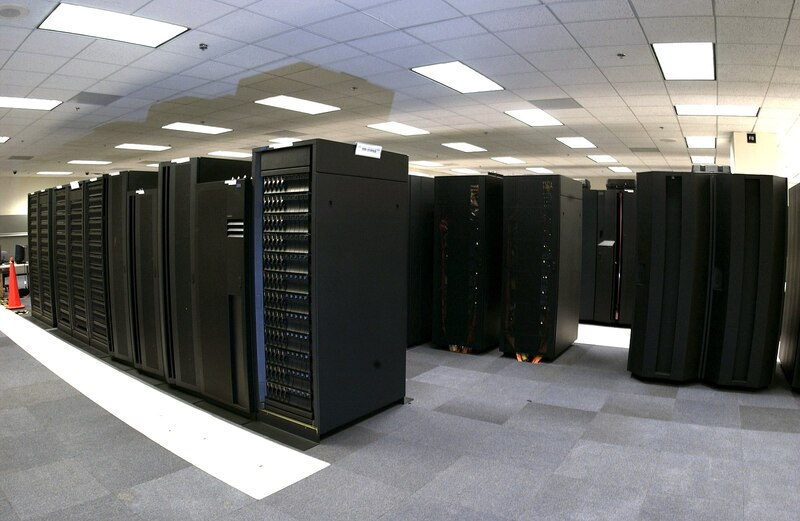
\includegraphics[width=76pt,height=46pt]{data-center.jpg}};
  \node at (2.7,-4.35) {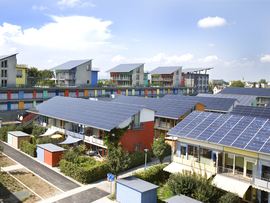
\includegraphics[width=76pt,height=46pt]{microgrid.jpg}}; 
  \draw[-latex] (2,-.25) to [in=45, out=-45] node[right] {Interactions} (2,-1.5);
  \draw[-latex] (-2,-1.5) to [out=135, in=-135] node[left] {Interactions} (-2,-.25);s
\end{tikzpicture}
\end{document}
